%\documentclass[spanish]{beamer}
\documentclass{beamer}
\usepackage{pgf,pgfpages}
%\pgfpagesuselayout{4 on 1}[letterpaper,landscape,border shrink=0.5in]
\usepackage{algorithm,algorithmic}
%\usepackage{algorithm,algorithmicx}
%\usepackage[noend]{algpseudocode}
\usepackage{listings}
\lstset{basicstyle=\ttfamily,
	showstringspaces=false,
	commentstyle=\color{red},
	literate={á}{{\'a}}1
	{ã}{{\~a}}1
	{é}{{\'e}}1
	{É}{{\'E}}1
	{ó}{{\'o}}1
	{í}{{\'i}}1
	{ñ}{{\~n}}1
	{¡}{{!`}}1
	{¿}{{?`}}1
	{ú}{{\'u}}1
	{Í}{{\'I}}1
	{Ó}{{\'O}}1
}

\usepackage{beamerthemesplit}
\usepackage{color}
\usepackage[utf8]{inputenc}
\usepackage[spanish]{babel}
%\usepackage[latin1]{inputenc}
%\usepackage[pdftex]{graphicx}
%\usepackage{algorithm}
%\usepackage{algorithmic-C}
%\usepackage{algorithmic}
\usepackage{amsthm}
\usepackage{multicol}
\usepackage{multirow}
\usepackage{fancyvrb,relsize}
\usepackage{hhline}
\usepackage{tikz}
\usetikzlibrary{trees, shapes, calc}
\newcommand{\inputTikZ}[2]{%
	\scalebox{#1}{\input{#2}}
}

\usetheme{Warsaw} %Gueno
%\usetheme{Darmstadt} %OK!
% \usetheme{Frankfurt} %OK!
%\usetheme{Goettingen}
%\usetheme{Dresden}
%\usetheme{JuanLesPins} %OK!!
%\usetheme{Marburg}
%\usetheme{Montpellier}
%\usetheme{Rochester} %sobrio
%\usetheme{Singapore}
%\usetheme{Szeged}

%\usecolortheme{albatross}
%\usecolortheme{seahorse}
%\usecolortheme{beetle}
%\usecolortheme{crane}
%\usecolortheme{dolphin}
%\usecolortheme{dove}
%\usecolortheme{fly}
%\usecolortheme{lily} %Gueno
\usecolortheme{orchid}%Gueno
%\usecolortheme{rose}
%\usecolortheme{seagull}
%\usecolortheme{whale}


\DefineVerbatimEnvironment%
      {VerbatimNN}%
      {Verbatim}%
      {fontsize=\relsize{-1}}
\DefineVerbatimEnvironment%
      {VerbatimNNN}%
      {Verbatim}%
      {fontsize=\relsize{-2}}

\DefineVerbatimEnvironment%
      {VerbatimPseudo}%
      {Verbatim}%
      {numbers=left, fontsize=\relsize{-1}}
\DefineVerbatimEnvironment%
      {VerbatimPseudoReduced}%
      {Verbatim}%
      {numbers=left, fontsize=\relsize{-2}}
\DefineVerbatimEnvironment%
      {VerbatimPseudoReduced2}%
      {Verbatim}%
      {numbers=left, fontsize=\relsize{-3}}
\DefineVerbatimEnvironment%
      {VerbatimC}%
      {Verbatim}%
      {commandchars=@ªº, numbers=left, fontsize=\relsize{-1}}
\DefineVerbatimEnvironment%
      {VerbatimReducedC}%
      {Verbatim}%
      {commandchars=@ªº, numbers=left, fontsize=\relsize{-2}}
\DefineVerbatimEnvironment%
      {VerbatimReduced2C}%
      {Verbatim}%
      {commandchars=@ªº, numbers=left, fontsize=\relsize{-3}}



%\AtBeginSubsection[]
%{
% \begin{frame}
% \frametitle{Sinopsis}
% Aqui decides: cada seccion y subseccion:
% \tableofcontents[currentsection,currentsubsection]
 %O solamente la seccion (Solo uno de ellos)
%\tableofcontents[currentsection]
% \end{frame}
%}

% Si quieres que todo por default aparezca de poco en poco
% descomenta esta linea
%\beamerdefaultoverlayspecification{<+->}

\setbeamertemplate{footline}{\hfill\insertframenumber/\inserttotalframenumber}
\setbeamertemplate{navigation symbols}{}

\setbeamercovered{transparent}

\title{ELO320 - Estructuras de Datos y Algoritmos\\HeapSort\\\small{Colas de Prioridad}}
%\subtitle{Ingeniería Civil Telemática UTFSM}
\author{Dr. Nicolás Gálvez R.\\{\small nicolas.galvez@usm.cl}}
\institute{Ing. Civil Telemática - Departamento de Electrónica}
\titlegraphic{
\includegraphics[scale=.14]{images/logoutfsm}}
\date{1er Semestre 2025}

\begin{document}

\frame{\titlepage}

%\section*{Sinopsis}
%\frame{  \frametitle{Sinopsis}\tableofcontents[pausesections]}
%
%
\part{Clase Activa}
\section{Clase Activa}
\begin{frame}[fragile]{Clase Activa: Módulo 1}
\begin{exampleblock}{Ejercicio 1.1}
\begin{itemize}
\item ¿Qué es un HEAP?
\item En un MIN-HEAP, asumiendo que todos los elementos son distintos, ¿dónde es posible encontrar el elemento con el menor valor y por qué?
\item Un arreglo con todos sus elementos en orden, ¿puede ser un MIN-HEAP? ¿Por qué? 
\item Un arreglo con los siguientes valores \{23; 17; 14; 6; 13; 10; 1; 5; 7; 12\} ¿puede ser un MAX-HEAP?
\end{itemize}
\end{exampleblock}
\end{frame}


\begin{frame}[fragile]{Clase Activa: Módulo 1}
\begin{exampleblock}{Ejercicio 1.2}
\begin{itemize}
\item Dibuje la operación de \texttt{heapify} en la posición 3 en el siguiente arreglo A = \{27; 17; 3; 16; 13; 10; 1; 5; 7; 12; 4; 8; 9; 0\}.
\item Transcriba \texttt{heapify} para un heap que utiliza MIN-HEAP.
\item ¿Cuál es el resultado de invocar a \texttt{heapify} cuando el elemento A[i] es mayor que sus hijos?
\item Transcriba \texttt{heapify} usando ciclos sin recursividad.
\end{itemize}
\end{exampleblock}
\end{frame}


\begin{frame}[fragile]{Clase Activa: Módulo 1}
\begin{exampleblock}{Ejercicio 1.3}
\begin{itemize}
\item Transcriba el código de \texttt{heapsort} usando MIN-HEAP.
\item Ordene de mayor a menor el arreglo A = \{27; 17; 3; 16; 13; 10; 1; 5; 7; 12; 4; 8; 9; 0\}, usando HeapSort.
\item Ordene de menor a mayor el arreglo A = \{27; 17; 3; 16; 13; 10; 1; 5; 7; 12; 4; 8; 9; 0\}, usando HeapSort.
\item ¿Cuál es la complejidad de HeapSort? ¿Por qué?. 
\end{itemize}
\end{exampleblock}
\end{frame}


\begin{frame}[fragile]{Clase Activa: Módulo 2}
\begin{exampleblock}{Ejercicio 2.1}
Considerando una Cola de Prioridad, basada en arreglos, programe:
\begin{itemize}
\item \texttt{get\_heap}: Retorna el valor del máximo valor en la cola.
\item \texttt{pop\_heap}: Retorna y remueve el valor máximo en la cola. 
\item \texttt{increase\_key}: Actualiza el valor de prioridad de un elemento, y reordena el heap de tal forma de mantener sus reglas. 
\item \texttt{insert\_key}: Añade un nuevo valor a la cola, y la ordena de tal forma de mantener las reglas del heap.
\end{itemize}
\end{exampleblock}
\end{frame}


\begin{frame}
\centering \Huge Información de Vital Importancia para la Clase Activa\footnote{Depende exclusivamente de uds. leerla y comprenderla.}.
\end{frame}

\part{HeapSort}
\section{HeapSort}
\begin{frame}[fragile]
 \frametitle{HeapSort}
\small Es un algoritmo de ordenamiento de complejidad $\mathcal{O}(n \log n)$, que combina la complejidad de MergeSort (se basa en un árbol binario) y la inserción \textit{in-place} de InsertSort.\\
\bigskip
HeapSort se basa en una estructura de datos llamada \textbf{Heap} (que no es la memoria):
\begin{itemize}
\item Árbol binario.
\item Árbol completo $\rightarrow$ $k-1$ niveles llenos, nivel $k$ parcial (izq. a der.).
\item Padres $>$ Hijos $\rightarrow$ MAX-HEAP.
\item Padres $<$ Hijos $ \rightarrow$ MIN-HEAP.
\end{itemize}
\bigskip
Nosotros \textbf{visualizaremos} un arreglo como un Heap, vale decir, \textbf{no crearemos un árbol}. Trabajaremos en el arreglo como si lo fuera.

\end{frame}

\begin{frame}[fragile]
 \frametitle{HeapSort: Heap}
\small
\begin{center}
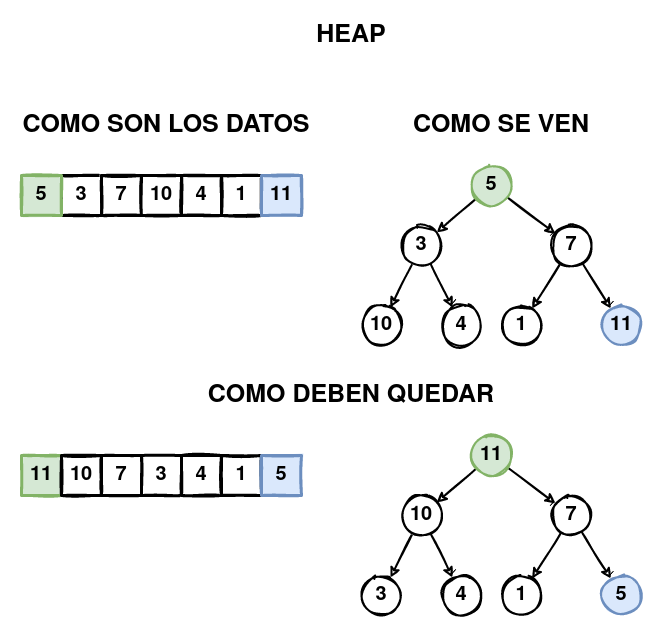
\includegraphics[width=0.7\linewidth]{images/heapsort/heap}
\end{center}
\end{frame}

\begin{frame}[fragile]
 \frametitle{HeapSort: Heap}
\small
La estructura del árbol depende de los índices del arreglo. Así, la \textbf{visualización} es fácil de establecer.

\begin{center}
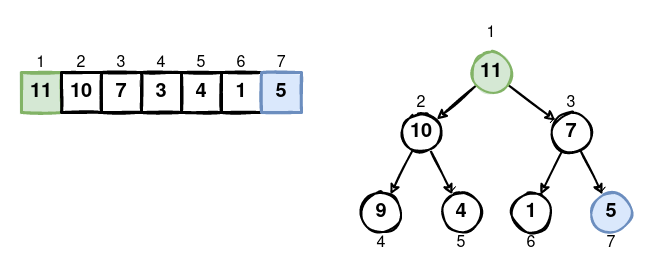
\includegraphics[width=0.8\linewidth]{images/heapsort/max-heap1}
\end{center}

Noten, que estamos trabajando con índices a partir del \textbf{número 1}, para simplificar la implementación. 
\end{frame}

\begin{frame}[fragile]
 \frametitle{HeapSort: Heap}
\small
\begin{exampleblock}{Funciones útiles}
\begin{lstlisting}[language=C, basicstyle=\tiny, escapeinside={|}{|}]
int padre(int i){ //padre del nodo con índice i
	return i/2; //div. entera (o usar floor de math.h)
}

int hijo_izq(int i){ //hijo izq del nodo con índice i
	return 2*i;
}

int hijo_der(int i){ //hijo der del nodo con índice i
	return (2*i)+1
}

\end{lstlisting}
\end{exampleblock}
\end{frame}

\begin{frame}[fragile]
 \frametitle{HeapSort: Heap}

\begin{center}
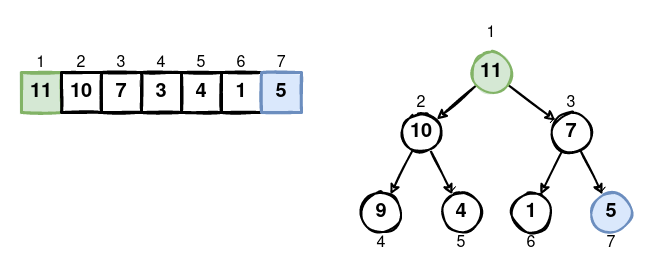
\includegraphics[width=0.8\linewidth]{images/heapsort/max-heap1}
\end{center}

\end{frame}


\begin{frame}[fragile]
 \frametitle{HeapSort: Heap}
\small \bigskip 
\noindent En esta clase nos centraremos en MAX-HEAP. 

\begin{center}
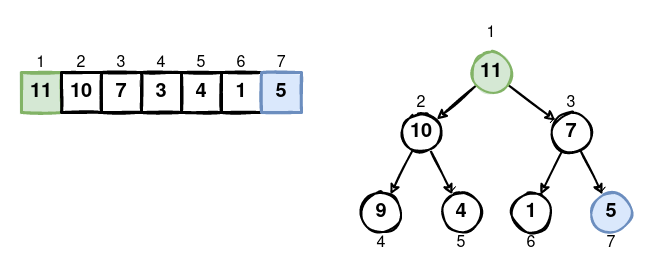
\includegraphics[width=0.7\linewidth]{images/heapsort/max-heap1}
\end{center}

\begin{center}
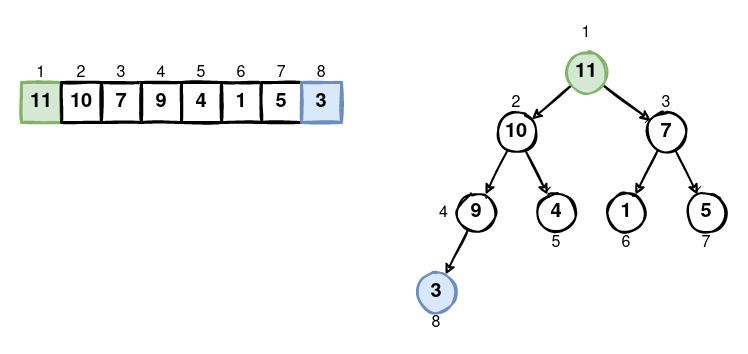
\includegraphics[width=0.7\linewidth]{images/heapsort/max-heap2}
\end{center}

\end{frame}

\begin{frame}[fragile]
 \frametitle{HeapSort: Heap}
\small \bigskip 
\noindent Noten que:
\begin{itemize}
\item El inicio del arreglo (raíz del árbol), será el mayor valor. 
\item El final del arreglo, será el nodo más a la derecha del último nivel (incompleto).
\end{itemize}

\begin{center}
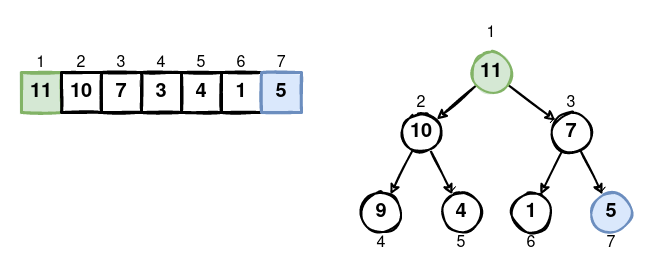
\includegraphics[width=0.55\linewidth]{images/heapsort/max-heap1}
\end{center}

\begin{center}
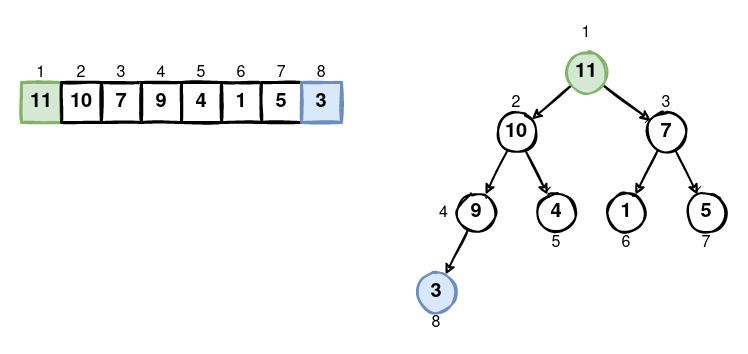
\includegraphics[width=0.55\linewidth]{images/heapsort/max-heap2}
\end{center}
\end{frame}

\begin{frame}[fragile]
 \frametitle{HeapSort: Componentes}
\small HeapSort se puede dividir en tres procedimientos: 
\begin{itemize}
\item \texttt{heapify}: Función recursiva que permite mantener las reglas del heap. Es de complejidad $\mathcal{O}(\log n)$.
\item \texttt{build\_heap}: Función que permite dejar el arreglo completo en formato MAX-HEAP o MIN-HEAP. Es lineal ($\mathcal{O}(n)$).
\item \texttt{HeapSort}: Procedimiento que ordena los datos utilizando las características del heap establecido. Es $\mathcal{O}(n \log n)$. 
\end{itemize}

\end{frame}


\begin{frame}[fragile]
 \frametitle{HeapSort: Heapify}

\begin{center}
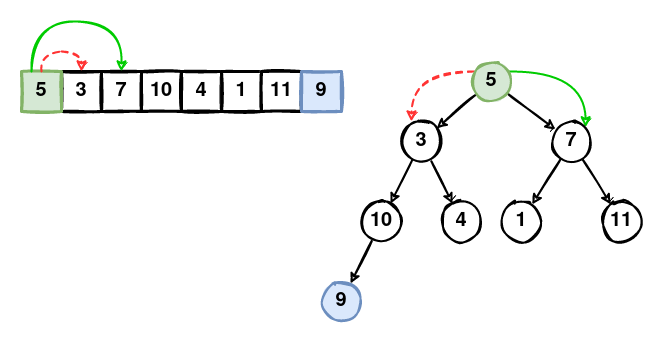
\includegraphics[width=0.8\linewidth]{images/heapsort/heapify1}
\end{center}

\end{frame}

\begin{frame}[fragile]
 \frametitle{HeapSort: Heapify}

\begin{center}
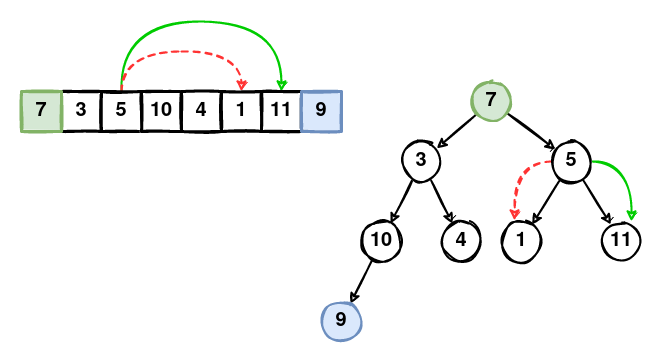
\includegraphics[width=0.8\linewidth]{images/heapsort/heapify2}
\end{center}

\end{frame}

\begin{frame}[fragile]
 \frametitle{HeapSort: Heapify}

\begin{center}
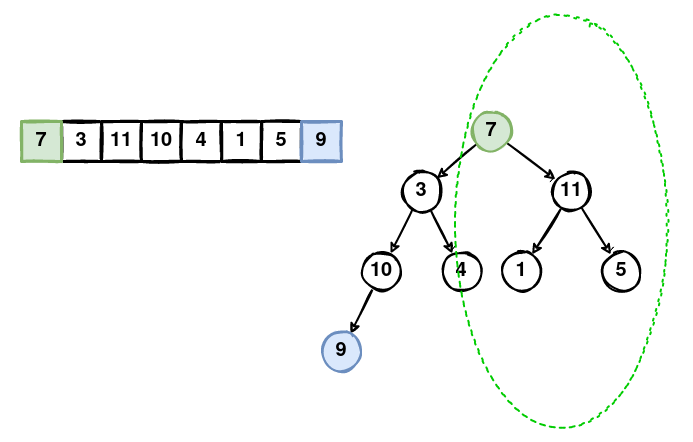
\includegraphics[width=0.8\linewidth]{images/heapsort/heapify3}
\end{center}

\end{frame}


\begin{frame}[fragile]
 \frametitle{HeapSort: Heapify}

\begin{exampleblock}{Heapify}
\begin{lstlisting}[language=C, basicstyle=\tiny, escapeinside={|}{|}]
void heapify(int arr[], int i, int tam){ //arreglo, índice, tamaño
    int mayor = i; //al inicio el nodo es el mayor
    int l = hijo_izq(i); 
    int r = hijo_der(i); 
 
    if (l < tam && arr[l] > arr[mayor]) //si no nos pasamos del largo
        mayor = l;			//y el padre es menor que el hijo izq
 
    if (r < tam && arr[r] > arr[mayor]) //luego la comparación con el hijo der
        mayor = r;
 
    if (mayor != i){ //intercambio
	int temp = arr[i];
	arr[i] = arr[mayor];
        arr[mayor] = temp;
 
        heapify(arr, mayor, tam); //recursividad sub-árbol
    }
}
\end{lstlisting}
\end{exampleblock}
\end{frame}

\begin{frame}[fragile]
 \frametitle{HeapSort: Build Heap}

\begin{center}
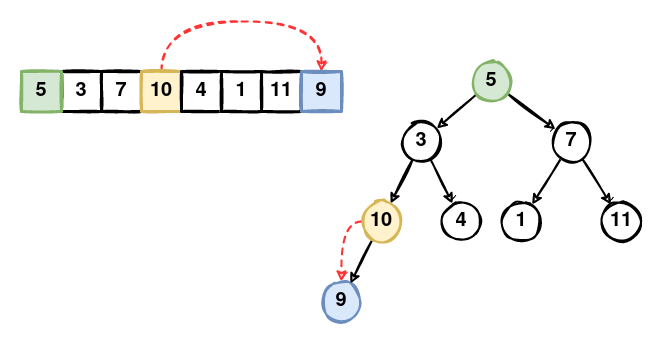
\includegraphics[width=0.8\linewidth]{images/heapsort/build-heap1}
\end{center}

\end{frame}

\begin{frame}[fragile]
 \frametitle{HeapSort: Build Heap}

\begin{center}
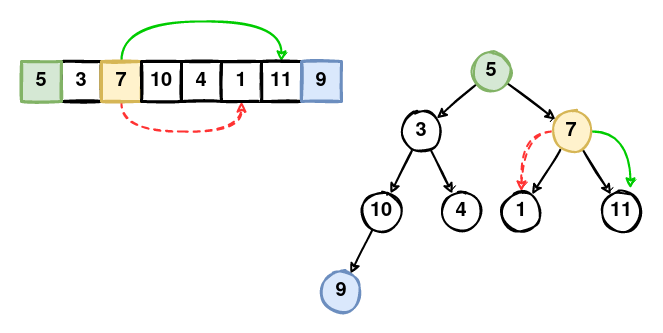
\includegraphics[width=0.8\linewidth]{images/heapsort/build-heap2}
\end{center}

\end{frame}

\begin{frame}[fragile]
 \frametitle{HeapSort: Build Heap}

\begin{center}
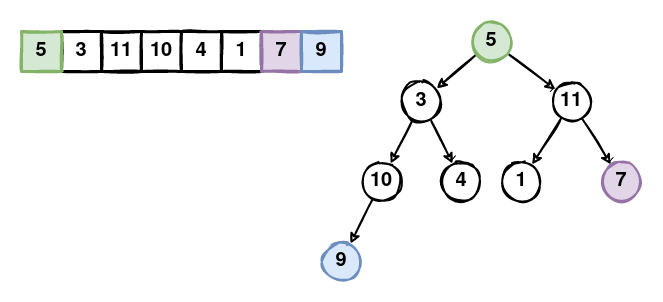
\includegraphics[width=0.8\linewidth]{images/heapsort/build-heap3}
\end{center}

\end{frame}

\begin{frame}[fragile]
 \frametitle{HeapSort: Build Heap}

\begin{center}
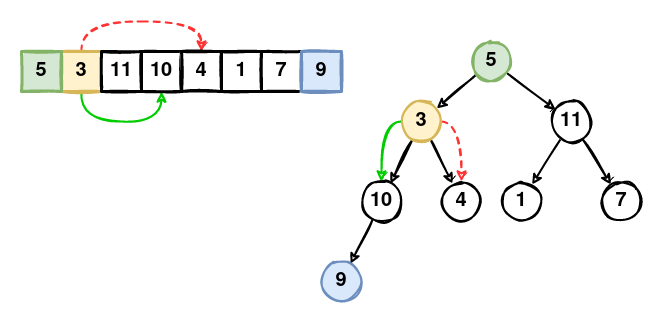
\includegraphics[width=0.8\linewidth]{images/heapsort/build-heap4}
\end{center}

\end{frame}

\begin{frame}[fragile]
 \frametitle{HeapSort: Build Heap}

\begin{center}
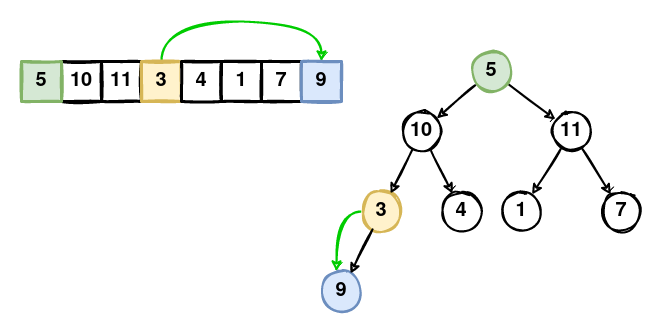
\includegraphics[width=0.8\linewidth]{images/heapsort/build-heap5}
\end{center}

\end{frame}

\begin{frame}[fragile]
 \frametitle{HeapSort: Build Heap}

\begin{center}
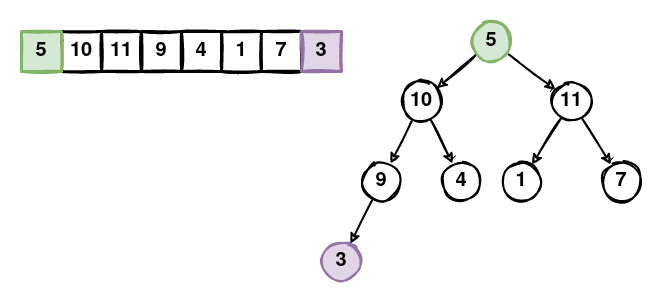
\includegraphics[width=0.8\linewidth]{images/heapsort/build-heap6}
\end{center}

\end{frame}

\begin{frame}[fragile]
 \frametitle{HeapSort: Build Heap}

\begin{center}
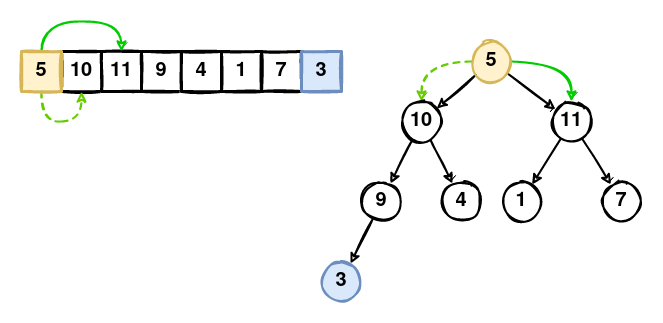
\includegraphics[width=0.8\linewidth]{images/heapsort/build-heap7}
\end{center}

\end{frame}

\begin{frame}[fragile]
 \frametitle{HeapSort: Build Heap}

\begin{center}
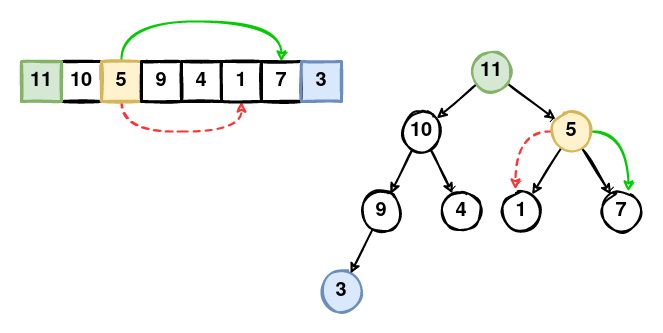
\includegraphics[width=0.8\linewidth]{images/heapsort/build-heap8}
\end{center}

\end{frame}

\begin{frame}[fragile]
 \frametitle{HeapSort: Build Heap}

\begin{center}
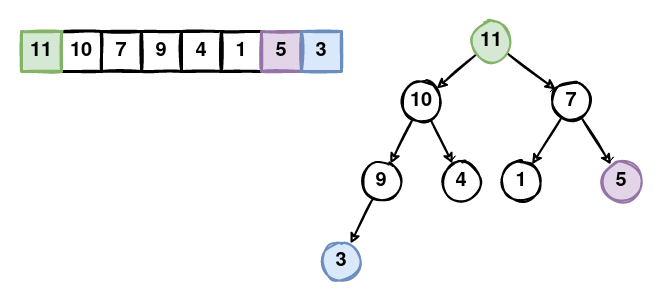
\includegraphics[width=0.8\linewidth]{images/heapsort/build-heap9}
\end{center}

\end{frame}


\begin{frame}[fragile]
 \frametitle{HeapSort: Build Heap}

\begin{exampleblock}{Build Heap}
\begin{lstlisting}[language=C, basicstyle=\tiny, escapeinside={|}{|}]
void build_heap(int arr[], int tam){ //arreglo y tamaño

	int i; 
	for (i=tam/2; i>0; i--){
		heapify(arr, i, tam);
	}
}
\end{lstlisting}
\end{exampleblock}
\end{frame}

\begin{frame}[fragile]
 \frametitle{HeapSort}

\begin{center}
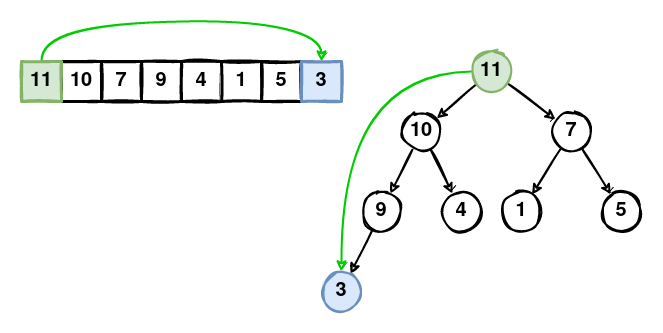
\includegraphics[width=0.8\linewidth]{images/heapsort/HeapSort1}
\end{center}

\end{frame}

\begin{frame}[fragile]
 \frametitle{HeapSort}

\begin{center}
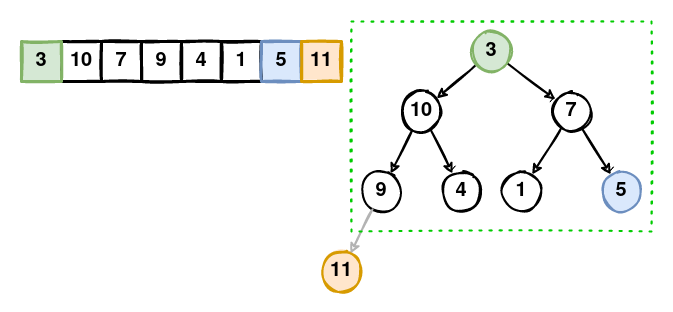
\includegraphics[width=0.8\linewidth]{images/heapsort/HeapSort2}
\end{center}

\end{frame}

\begin{frame}[fragile]
 \frametitle{HeapSort}

\begin{center}
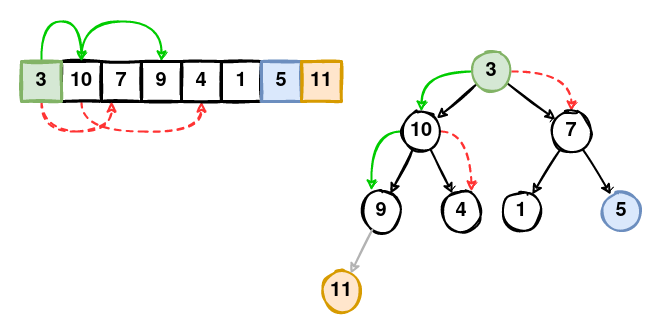
\includegraphics[width=0.8\linewidth]{images/heapsort/HeapSort3}
\end{center}

\end{frame}

\begin{frame}[fragile]
 \frametitle{HeapSort}

\begin{center}
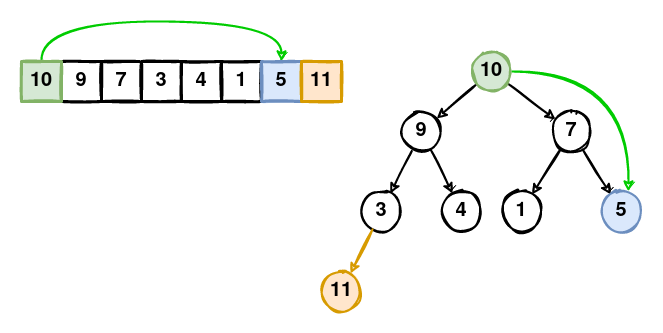
\includegraphics[width=0.8\linewidth]{images/heapsort/HeapSort4}
\end{center}

\end{frame}

\begin{frame}[fragile]
 \frametitle{HeapSort}

\begin{center}
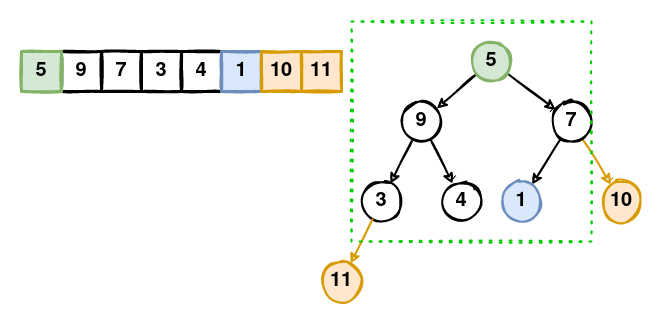
\includegraphics[width=0.8\linewidth]{images/heapsort/HeapSort5}
\end{center}

\end{frame}

\begin{frame}[fragile]
 \frametitle{HeapSort}

\begin{center}
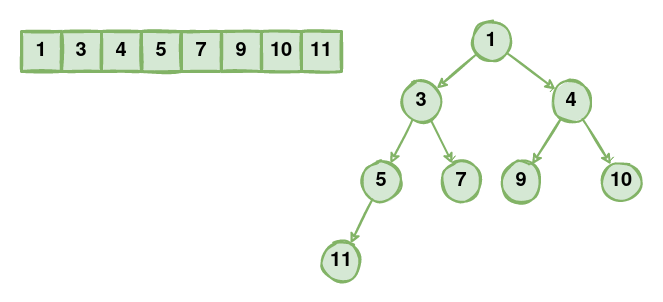
\includegraphics[width=0.8\linewidth]{images/heapsort/HeapSort6}
\end{center}

\end{frame}

\begin{frame}[fragile]
 \frametitle{HeapSort}

\begin{exampleblock}{HeapSort}
\begin{lstlisting}[language=C, basicstyle=\tiny, escapeinside={|}{|}]
void HeapSort(int arr[], int tam){ //arreglo y tamaño

	int temp;

	build_heap(arr, tam);

	for (int i = tam; i > 1; i--){//cada vuelta el tamaño (i) baja en 1.
		temp=arr[1]; //dar vuelta primero con último
		arr[i] = arr[1];
		arr[1] = temp;

	        heapify(arr, 1, i-1); //arreglar el heap post-cambio
    	}

}
\end{lstlisting}
\end{exampleblock}
\end{frame}

\section{Colas de Prioridad}
\begin{frame}[fragile]
 \frametitle{Colas de Prioridad}
\small La estructura del heap (binary heap), es bastante utilizada, siendo su mayor aplicación las \textbf{Colas de Prioridad}. \\

En una cola de prioridad, datos son asociados con un valor (entero) representando su prioridad, y son ordenados según ésta. 

\begin{itemize}
\item Schedulers de clúster (qsub, sbatch, etc).
\item Prioridad de procesos (Task Manager, PID priority).
\end{itemize}

Se utiliza una cola con MAX-HEAP, la cual es fácilmente implementada en un arreglo. 
\end{frame}

\begin{frame}[fragile]
 \frametitle{Colas de Prioridad: Operaciones básicas}
\small 

\begin{itemize}
\item \texttt{get\_heap}: Retorna el valor del máximo valor en la cola.
\item \texttt{pop\_heap}: Retorna y remueve el valor máximo en la cola. 
\item \texttt{increase\_key}: Actualiza el valor de prioridad de un elemento, y reordena el heap de tal forma de mantener sus reglas. 
\item \texttt{insert\_key}: Añade un nuevo valor a la cola, y la ordena de tal forma de mantener las reglas del heap.
\end{itemize}


\begin{itemize}
\item \texttt{get\_heap}: $\mathcal{O}(1)$.
\item \texttt{pop\_heap}: $\mathcal{O}(\log n)$.
\item \texttt{increase\_key}: $\mathcal{O}(\log n)$.
\item \texttt{insert\_key}: $\mathcal{O}(\log n)$. 
\end{itemize}

\end{frame}


%\section{Ejercicios}
%\begin{frame}[fragile]
% \frametitle{HeapSort}
%\small
%\begin{itemize}
%\item Dibuje e implemente el proceso de cada uno de los métodos de cola de prioridad.
%\item En un MAX-HEAP, asumiendo que todos los elementos son distintos, ¿dónde es posible encontrar el elemento con el menor valor y por qué?
%\item Un arreglo con todos sus elementos en orden, ¿puede ser un MIN-HEAP? ¿Por qué? 
%\item Un arreglo con los siguientes valores \{23; 17; 14; 6; 13; 10; 1; 5; 7; 12\} ¿puede ser un MAX-HEAP?
%\item Dibuje  la operación de \texttt{heapify} en la posición 3 en el siguiente arreglo A = \{27; 17; 3; 16; 13; 10; 1; 5; 7; 12; 4; 8; 9; 0\}.
%\item Transcriba \texttt{heapify} para un heap que utiliza MIN-HEAP.
%\item ¿Cuál es el resultado de invocar a \texttt{heapify} cuando el elemento A[i] es mayor que sus hijos?
%\item Transcriba \texttt{heapify} usando ciclos sin recursividad.
%\end{itemize}
%\end{frame}
%\section{Recuento: Análisis de Complejidad}
%\begin{frame}[fragile]
% \frametitle{Tiempo de ejecución de un Algoritmo}
%\small Definiremos a $T(n)$ como la función de tiempo de ejecución de un algoritmo con input $n$, y la expresaremos en función a la cantidad de instrucciones.
%\bigskip
%Costo de las operaciones en unidades de tiempo [ut]:
%\begin{itemize}
%\item Instrucciones básicas: $1$
%\item Secuencia de $n$ instrucciones:  $c \times n = n$ (c: cte. de costo)
%\item if-else: $T(\text{condición}) + \text{max}\{T(\text{if}), T(\text{else})\}$
%\item while: $(n+1) \times T(\text{condición}) + n \times T(\text{while}) $
%\end{itemize}
%\end{frame}
%
%
%\begin{frame}[fragile]
% \frametitle{Tiempo de ejecución de un Algoritmo}
%\begin{exampleblock}{¿Cuál es la complejidad del siguiente algoritmo}
%\begin{lstlisting}[language=C, basicstyle=\tiny, escapeinside={|}{|}]
%int suma(int n) {
%	int sum = 0, i, j;
%	for (i=0; i < n; i++) 
%		for (j=0; j < n; j++)
%			sum++;
%	return sum;
%}
%\end{lstlisting}
%\end{exampleblock}
%\pause
%\begin{itemize}
%\item Número de iteraciones: \pause $n^2$. \pause
%\item Costo de cada iteración: \pause $3n+4$. \pause
%\item Costo total: \pause $((2n+2) \times (3n+2))+4 = 6n^2 + 10n + 8 $.
%\end{itemize}
%
%\end{frame}
%
%
%\begin{frame}[fragile]
% \frametitle{Complejidad Algorítmica vs Entorno de ejecución.}
%\small
%En esta unidad veremos algoritmos de ordenamiento, los primeros dos que veremos (más adelante) son:
%\begin{itemize}
%\item \textbf{Insert Sort}: $T_1(n) = c_1 \times n^2$
%\item \textbf{Merge Sort}: $T_2(n) = c_2 \times n \times \log{n}$
%\end{itemize}
%
%Supongamos que el PC-A está ejecutando \textbf{Insert Sort}, que el PC-B está ejecutando \textbf{Merge Sort} y que ambos deben ordenar un arreglo de 10 millones de enteros.
%Además, el PC-A es ultima generación y ejecuta 10 mil millones de instrucciones por segundo y el PC-B tiene 10 años de antigüedad, ergo solo procesa 10 millones de instrucciones por segundo.
%Incluyamos lo siguiente:
%\begin{itemize}
%\item Oliver Atom programó \textbf{Insert Sort} en el PC-A usando lenguaje de máquina (assembly) resultando en un costo de $2\times 2^n$ instrucciones para ordenar n números.
%\item El Corxea implementa \textbf{Merge Sort}, en el PC-B usando C++, con un compilador antiguo e ineficiente, y el código resultante toma $50 \times n \times \log{n}$ instrucciones para ordenar n números.
%\end{itemize}
%
%\end{frame}
%
%
%\begin{frame}[fragile]
% \frametitle{Complejidad Algorítmica vs Entorno de ejecución.}
%\small
%
%\begin{itemize}
%\item PC-A:
%$$ \frac{2 \times (10^7)^2}{10^{10}} = 20000\ [s]\ \ (>5.5 [h])$$
%\item PC-B:
%$$ \frac{50 \times 10^7 \times \log{10^7}}{10^{7}} \approx 1163\ [s]\ \ (< 20 [min])$$
%\end{itemize}
%\bigskip
%\textbf{PC-B completa su algoritmo 17 veces más rápido que el algoritmo usado en PC-A, siendo el primer entorno de ejecución 1000 veces más lento que el segundo}.
%
%\end{frame}
%
%\begin{frame}[fragile]
% \frametitle{Complejidad Algorítmica vs Entorno de ejecución.}
%\small
%
%\begin{center}
%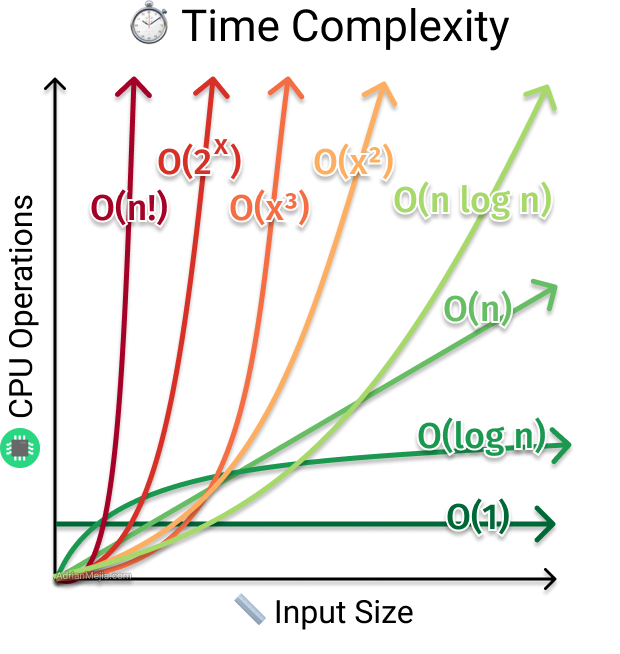
\includegraphics[width=.7\linewidth]{images/timecomplexity2}
%\end{center}
%
%
%\end{frame}
%
%\begin{frame}[fragile]
% \frametitle{Análisis Asintótico}
%\small Una vez entendido el análisis de tiempo buscaremos análisis asintótico de los algoritmos. En la práctica significa concentrarse en el término predominante en $T(n)$, y luego encontrar cotas superiores y/o inferiores de rendimiento.
%
%Existen tres notaciones asintóticas generalmente usadas:
%\begin{itemize}
%\item Big O ($\mathcal{O}$): Cota superior asintótica, vale decir, cota al peor desempeño.
%\item Big Omega ($\Omega$): Cota inferior asintótica, vale decir, cota al mejor desempeño.
%\item Big Theta ($\Theta$): Cota compuesta, vale decir, cota al rendimiento promedio. 
%\end{itemize}
%
%\bigskip
%Comúnmente, se utiliza la notación en peor escenario, vale decir, Big O ($\mathcal{O}$). 
%\end{frame}
%
%\section{Merge Sort}
%\begin{frame}[fragile]
% \frametitle{Merge Sort}
%\small
%Algoritmo de ordenamiento \textbf{recursivo} que aplica la técnica \textbf{Divide \& Conquer}.
%
%\begin{itemize}
%\item Peor escenario: $\mathcal{O}(n \log n)$
%\item Mejor escenario: $\Omega(n \log n)$
%\item Escenario Promedio: $\Theta(n \log n)$
%\end{itemize}
%
%Características:
%\begin{itemize}
%\item Estable y rápido, sobre todo para tamaños grandes de datos.
%\item Es superado en tamaños pequeños de datos.
%\item Necesita un espacio de memoria extra para el ordenamiento ($\Theta(n)$).
%\end{itemize}
%
%\end{frame}
%
%\section{Merge Sort}
%\begin{frame}[fragile]
% \frametitle{Merge Sort}
%\begin{center}
%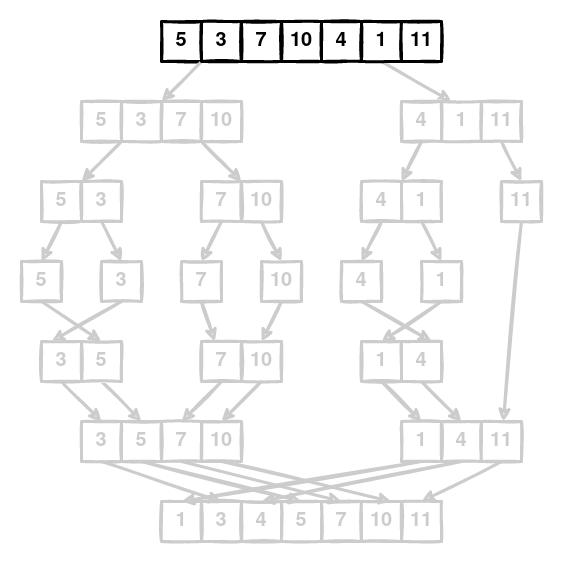
\includegraphics[width=.7\linewidth]{images/mergesort/MergeSort1}
%\end{center}
%\end{frame}
%
%\begin{frame}[fragile]
% \frametitle{Merge Sort}
%\begin{center}
%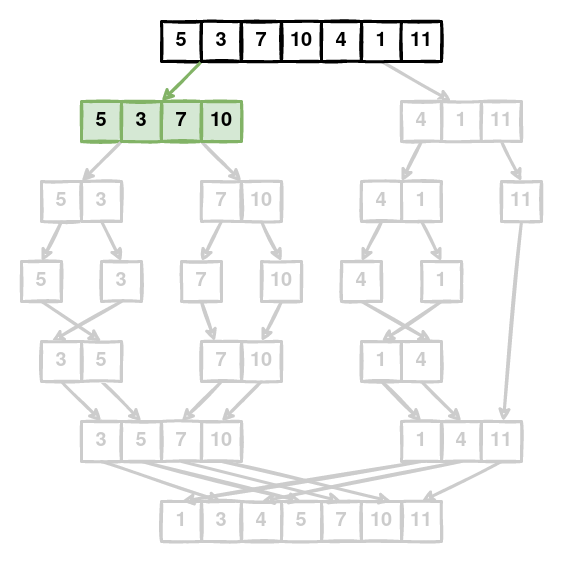
\includegraphics[width=.7\linewidth]{images/mergesort/MergeSort2}
%\end{center}
%\end{frame}
%
%\begin{frame}[fragile]
% \frametitle{Merge Sort}
%\begin{center}
%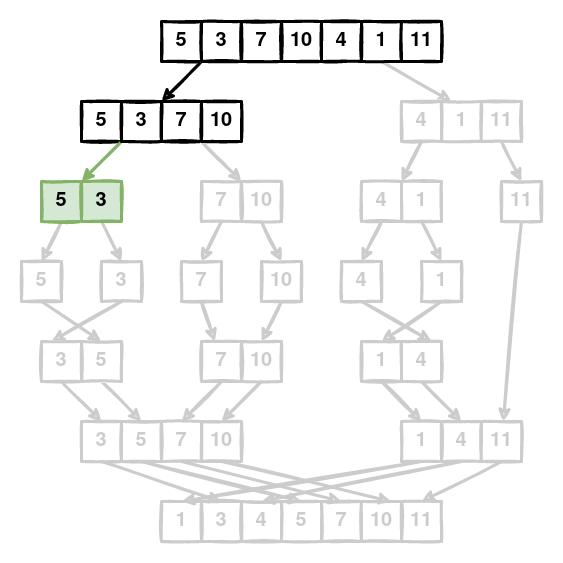
\includegraphics[width=.7\linewidth]{images/mergesort/MergeSort3}
%\end{center}
%\end{frame}
%
%\begin{frame}[fragile]
% \frametitle{Merge Sort}
%\begin{center}
%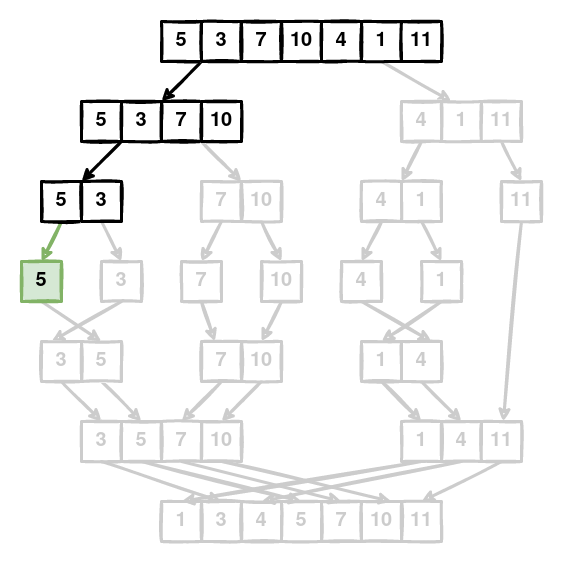
\includegraphics[width=.7\linewidth]{images/mergesort/MergeSort4}
%\end{center}
%\end{frame}
%
%\begin{frame}[fragile]
% \frametitle{Merge Sort}
%\begin{center}
%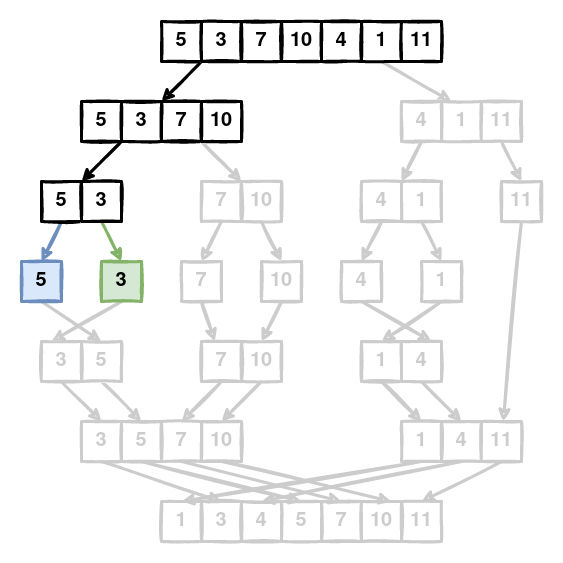
\includegraphics[width=.7\linewidth]{images/mergesort/MergeSort5}
%\end{center}
%\end{frame}
%
%\begin{frame}[fragile]
% \frametitle{Merge Sort}
%\begin{center}
%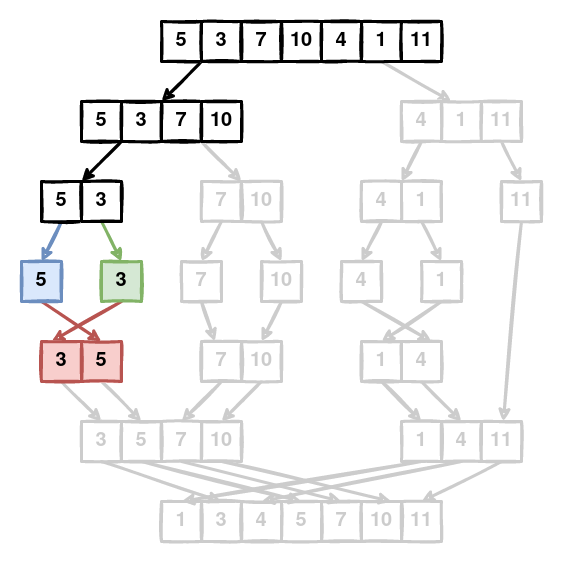
\includegraphics[width=.7\linewidth]{images/mergesort/MergeSort6}
%\end{center}
%\end{frame}
%
%\begin{frame}[fragile]
% \frametitle{Merge Sort}
%\begin{center}
%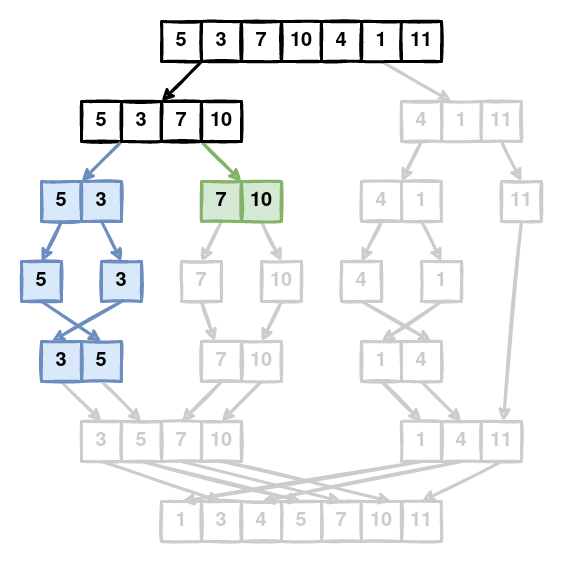
\includegraphics[width=.7\linewidth]{images/mergesort/MergeSort7}
%\end{center}
%\end{frame}
%
%\begin{frame}[fragile]
% \frametitle{Merge Sort}
%\begin{center}
%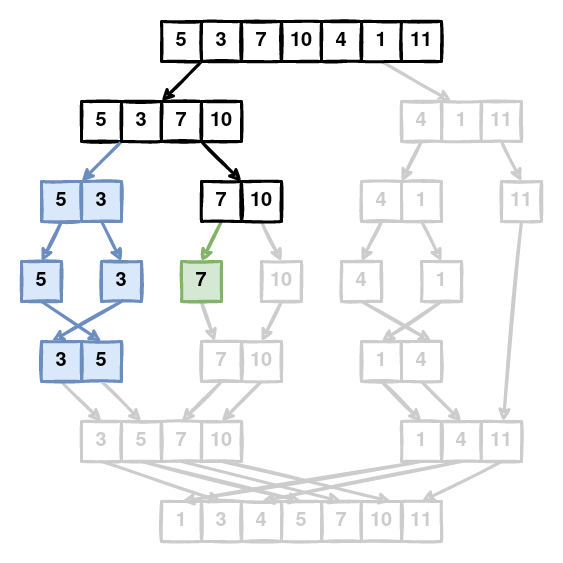
\includegraphics[width=.7\linewidth]{images/mergesort/MergeSort8}
%\end{center}
%\end{frame}
%
%\begin{frame}[fragile]
% \frametitle{Merge Sort}
%\begin{center}
%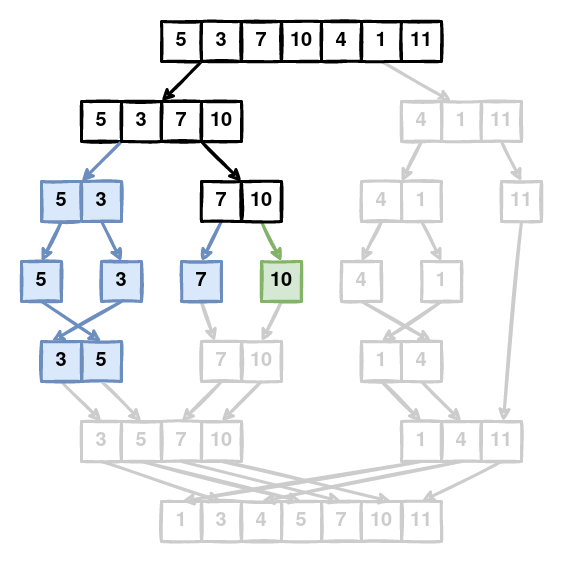
\includegraphics[width=.7\linewidth]{images/mergesort/MergeSort9}
%\end{center}
%\end{frame}
%
%\begin{frame}[fragile]
% \frametitle{Merge Sort}
%\begin{center}
%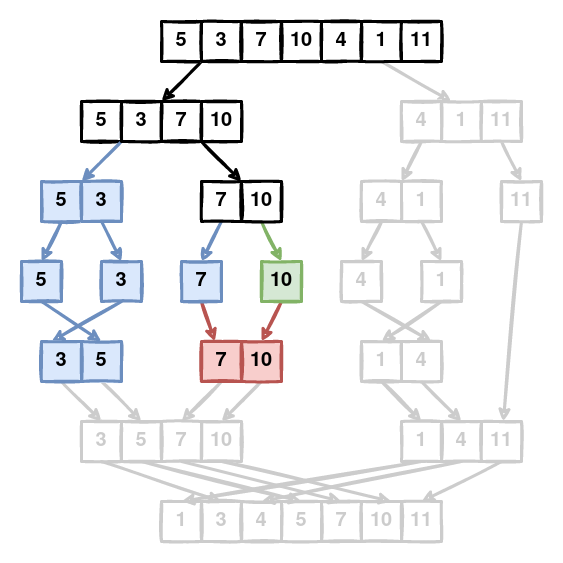
\includegraphics[width=.7\linewidth]{images/mergesort/MergeSort10}
%\end{center}
%\end{frame}
%
%\begin{frame}[fragile]
% \frametitle{Merge Sort}
%\begin{center}
%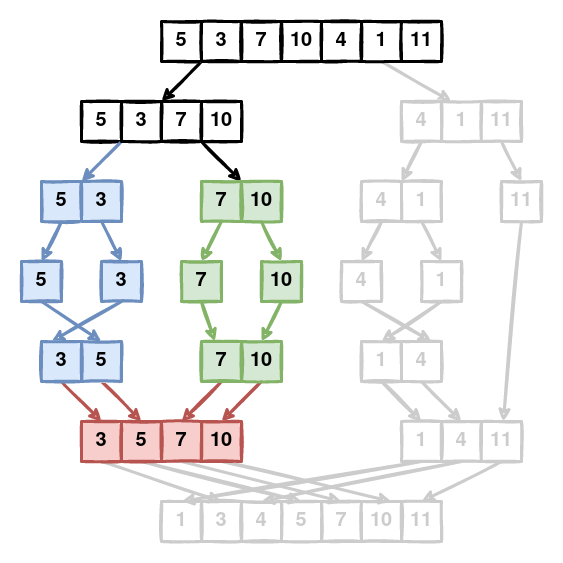
\includegraphics[width=.7\linewidth]{images/mergesort/MergeSort11}
%\end{center}
%\end{frame}
%
%\begin{frame}[fragile]
% \frametitle{Merge Sort}
%\begin{center}
%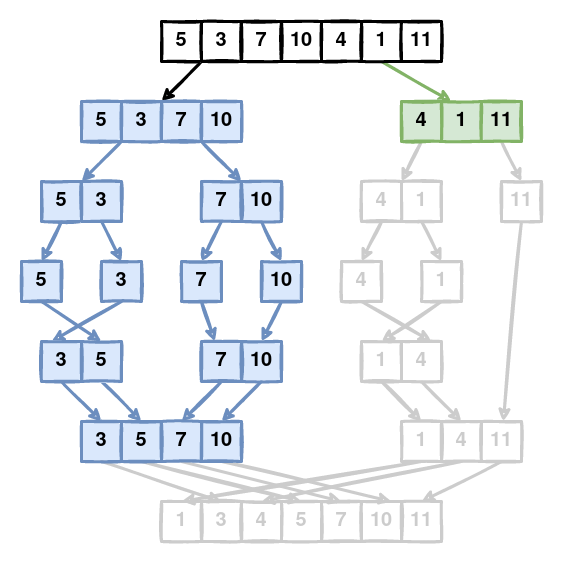
\includegraphics[width=.7\linewidth]{images/mergesort/MergeSort12}
%\end{center}
%\end{frame}
%
%\begin{frame}[fragile]
% \frametitle{Merge Sort}
%\begin{center}
%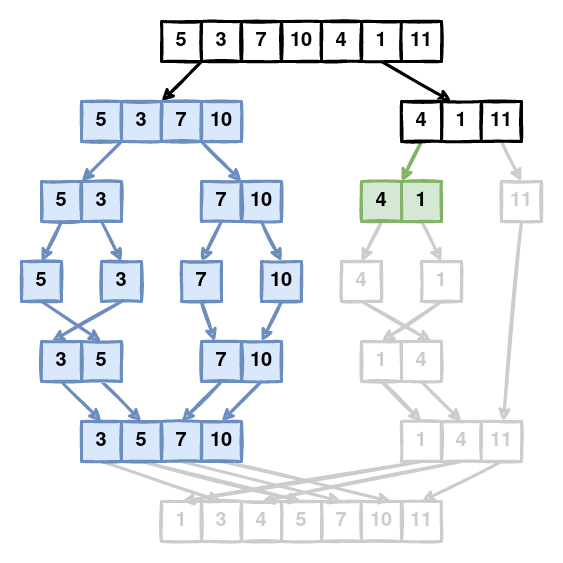
\includegraphics[width=.7\linewidth]{images/mergesort/MergeSort13}
%\end{center}
%\end{frame}
%
%\begin{frame}[fragile]
% \frametitle{Merge Sort}
%\begin{center}
%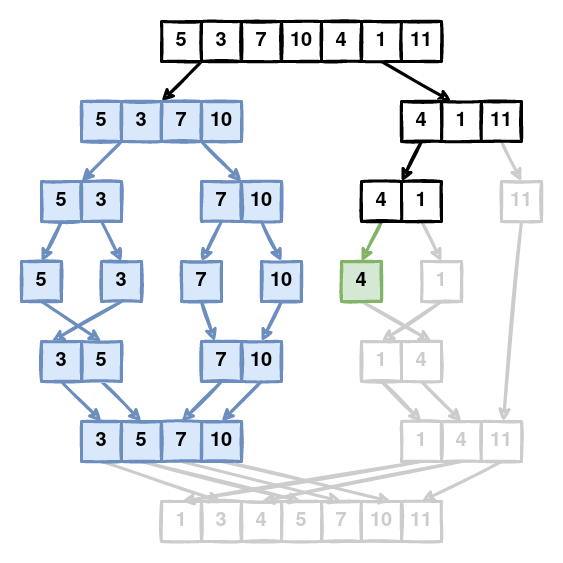
\includegraphics[width=.7\linewidth]{images/mergesort/MergeSort14}
%\end{center}
%\end{frame}
%
%\begin{frame}[fragile]
% \frametitle{Merge Sort}
%\begin{center}
%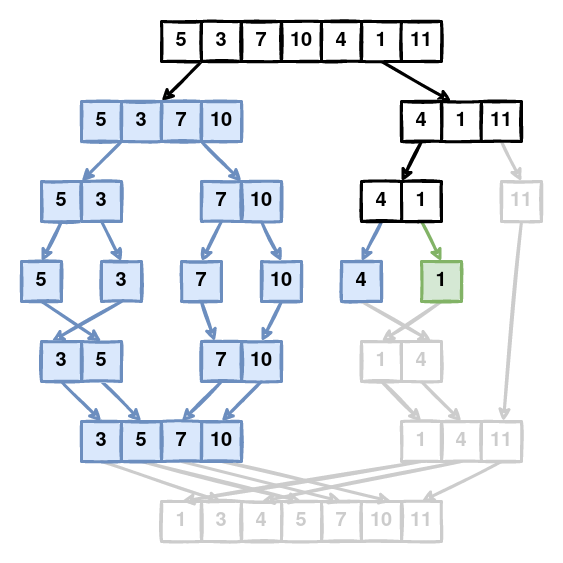
\includegraphics[width=.7\linewidth]{images/mergesort/MergeSort15}
%\end{center}
%\end{frame}
%
%\begin{frame}[fragile]
% \frametitle{Merge Sort}
%\begin{center}
%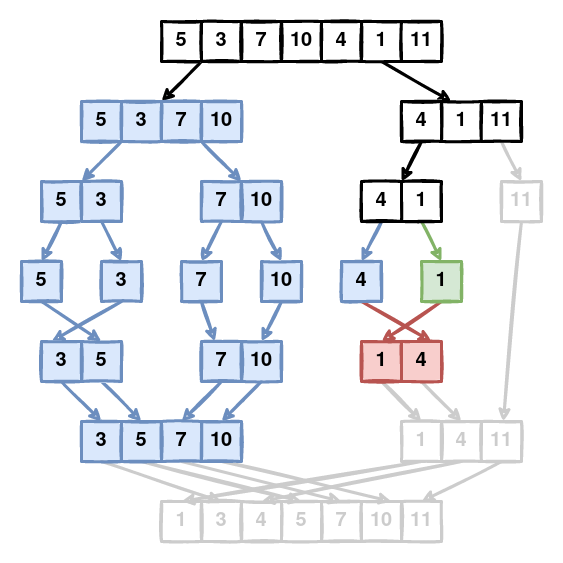
\includegraphics[width=.7\linewidth]{images/mergesort/MergeSort16}
%\end{center}
%\end{frame}
%
%\begin{frame}[fragile]
% \frametitle{Merge Sort}
%\begin{center}
%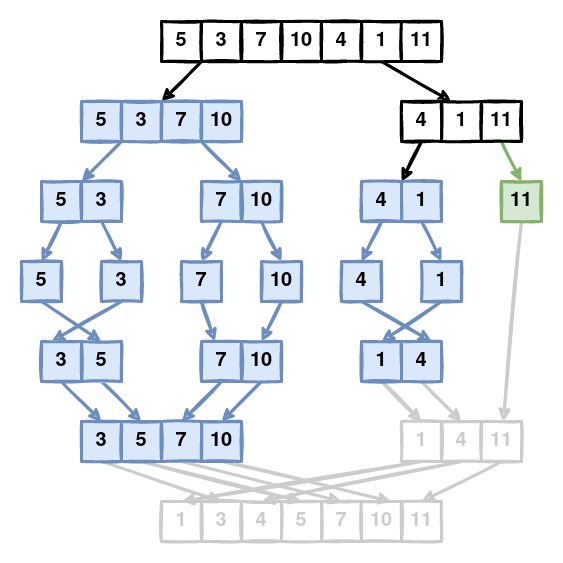
\includegraphics[width=.7\linewidth]{images/mergesort/MergeSort17}
%\end{center}
%\end{frame}
%
%\begin{frame}[fragile]
% \frametitle{Merge Sort}
%\begin{center}
%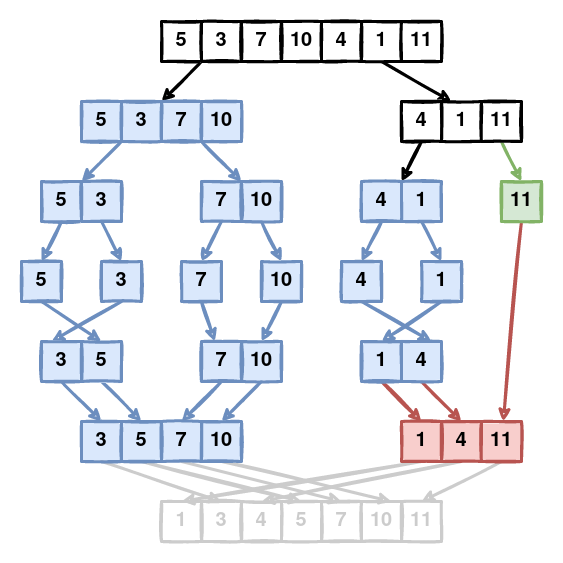
\includegraphics[width=.7\linewidth]{images/mergesort/MergeSort18}
%\end{center}
%\end{frame}
%
%\begin{frame}[fragile]
% \frametitle{Merge Sort}
%\begin{center}
%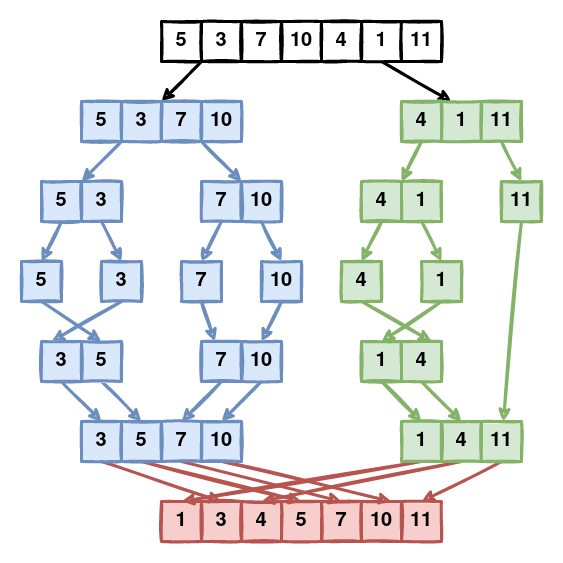
\includegraphics[width=.7\linewidth]{images/mergesort/MergeSort19}
%\end{center}
%\end{frame}
%
%\begin{frame}[fragile]
% \frametitle{Merge Sort}
%\begin{center}
%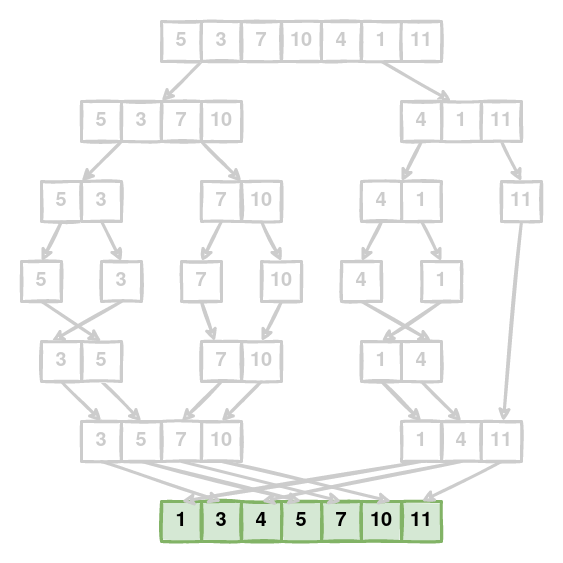
\includegraphics[width=.7\linewidth]{images/mergesort/MergeSort20}
%\end{center}
%\end{frame}
%
%\begin{frame}[fragile]
% \frametitle{MergeSort}
%\begin{exampleblock}{MergeSort}
%\begin{lstlisting}[language=C, basicstyle=\tiny, escapeinside={|}{|}]
%void mergeSort(int arr[], int l, int r){ //l=izq, r=der (indices)
%    if (l < r) {
%        int m = l + (r - l) / 2; //div. entera
%
%        mergeSort(arr, l, m); //dividir
%        mergeSort(arr, m + 1, r); //post-orden
%
%        merge(arr, l, m, r); //mezclar
%    }
%}
%\end{lstlisting}
%\end{exampleblock}
%\end{frame}
%
%\begin{frame}[fragile]
% \frametitle{MergeSort}
%\begin{exampleblock}{merge}
%\begin{lstlisting}[language=C, basicstyle=\tiny, escapeinside={|}{|}]
%void merge(int arr[], int l, int m, int r){
%    int i, j, k;
%    int n1 = m - l + 1;
%    int n2 = r - m;
%
%    int L[n1], R[n2]; //arreglos temporales
%
%    for (i = 0; i < n1; i++) //copia a los arreglos
%        L[i] = arr[l + i];
%    for (j = 0; j < n2; j++)
%        R[j] = arr[m + 1 + j];
%
%    i = 0; j=0; k = l; //mezcla
%    while (i<n1 && j<n2) {
%        if (L[i] <= R[j]) {
%            arr[k] = L[i]; i++;
%        }else{
%            arr[k] = R[j]; j++;
%        }
%        k++;
%    }
%
%    while (i < n1){ //si sobra de L
%        arr[k] = L[i]; i++; k++;
%    }
%
%    while (j < n2) { //si sobra de R
%        arr[k] = R[j]; j++; k++;
%    }
%}
%\end{lstlisting}
%\end{exampleblock}
%\end{frame}
%
%\section{Funciones de Recurrencia}
%\begin{frame}[fragile]
% \frametitle{Funciones de Recurrencia}
%\small
%¿Cómo podemos determinar la complejidad de MergeSort si éste trabaja recursivamente?
%\begin{itemize}
%\item Peor escenario: $\mathcal{O}(n \log n)$
%\item Mejor escenario: $\Omega(n \log n)$
%\item Escenario Promedio: $\Theta(n \log n)$
%\end{itemize}
%
%\textbf{Funciones de recurrencia}, relaciones matemáticas recursivas que son utilizadas en ciencias de la computación para explicar la complejidad de éste tipo de algoritmos.
%\end{frame}
%
%\begin{frame}[fragile]
% \frametitle{Funciones de Recurrencia}
%\small
%\begin{exampleblock}{Factorial}
%\begin{lstlisting}[language=C, basicstyle=\tiny, escapeinside={|}{|}]
%int factorial(int n){
%	if(n>0)
%		exit(-1);
%
%	if(n==0)
%		return 1;
%	return n * factorial(n-1); // 1 + T(n-1)
%}
%\end{lstlisting}
%\end{exampleblock}
%
%Sabemos:
%\begin{itemize}
%\item $T(n) = 1$ (si $n = 0$).
%\item $T(n) = 1 + T(n-1)$ (si $n > 0$).
%\item Luego: $T(n) = 1 + 1 + 1 + \dots + T(1) = n$.\pause
%\item $T(n) = n \rightarrow \mathcal{O}(n)$.
%\end{itemize}
%\end{frame}
%
%
%
%\begin{frame}[fragile]
% \frametitle{Funciones de Recurrencia}
%\small
%\begin{exampleblock}{Búsqueda Binaria}
%\begin{lstlisting}[language=C, basicstyle=\tiny, escapeinside={|}{|}]
%int binarySearch(int arr[], int l, int r, int x){
%    if (r >= l) {
%        int mid = l + (r - l) / 2;
%
%        if (arr[mid] == x) //if-else 1 + T(n/2)
%            return mid;
%
%        if (arr[mid] > x)
%            return binarySearch(arr, l, mid - 1, x);
%	return binarySearch(arr, mid + 1, r, x); //else
%    }
%
%    return -1;
%}
%\end{lstlisting}
%\end{exampleblock}
%
%
%\begin{itemize}
%\item $T(n) = 1$ (si $n = 1$).
%\item $T(n) = 1+ T(n/2) $ (si $n > 1$).
%\item Luego: $T(n) = 1 + 1 + 1 + \dots + T(n/2^k)$ \pause
%\item Al finalizar: $T(n/2^k) = T(1) \rightarrow n = 2^k$ \pause
%\item $\log_2 n  = log_2(2^k) \rightarrow k = \log_2 n $ \pause 
%\item $ T(n) = 1 + T(n/2) = 1 + \mathcal{O}(\log n) = \mathcal{O}(\log n)$
%\end{itemize}
%\end{frame}
%
%
%\begin{frame}[fragile]
% \frametitle{Funciones de Recurrencia}
%\small
%\begin{exampleblock}{MergeSort}
%\begin{lstlisting}[language=C, basicstyle=\tiny, escapeinside={|}{|}]
%void mergeSort(int arr[], int l, int r){ //l=izq, r=der (indices)
%    if (l < r) {
%        int m = l + (r - l) / 2; // |$\mathcal{O}(1)$|
%
%        mergeSort(arr, l, m); // T(n/2)
%        mergeSort(arr, m + 1, r); // T(n/2)
%
%        merge(arr, l, m, r); // |$\mathcal{O}(n)$| 
%    }
%}
%
%\end{lstlisting}
%\end{exampleblock}
%
%
%\begin{itemize}
%\item $T(n) = 1$ (si $n = 1$).
%\item $T(n) = n + 2 \times T(n/2) $ (si $n > 1$).
%\item $T(n) = n (1 + \log n) = n + n \log n$
%\item $T(n) = \mathcal{O}(n \log n) $
%\end{itemize}
%\end{frame}
%
%
%\begin{frame}[fragile]
% \frametitle{Funciones de Recurrencia: Ejercicios}
%\small
%Desarrolle las siguientes funciones de recurrencia, y determine su cota superior asintótica $\mathcal{O}(g(n))$ (tip: use árboles):
%\begin{itemize}
%\item $T(n) = T(n/2) + n^2$
%\item $T(n) = 4T((n/2) + 2) + n$
%\item $T(n) = 2T(n-1) + 1$
%\end{itemize}
%\end{frame}


\end{document}
